\sectionauthor[Simon Blom; Romy Schardam]{Evolution of Prototype Design}
% This chapter is where you document the entire journey of your prototype's development. It should not only showcase your final product but also the thoughtful and iterative process that led to its creation. This narrative should be detailed and reflective, offering a comprehensive and transparent view of your design process. This chapter is your opportunity to demonstrate your team's problem-solving skills, adaptability, and ability to integrate feedback into a practical solution.
% \begin{itemize}
%     \item Step-by-Step Evolution: Describe each stage of your prototype's development. This should include the initial concept, any interim versions, and the final design. For each step, explain the rationale behind the design choices made, focusing on both the successes and challenges you encountered.
%     \item Design Motivation: Detail the motivations for each design change. These motivations can be varied - they might stem from your own insights, experimentation, feedback from stakeholders, or new information from scientific literature. It's important to articulate why each change was made and how it contributes to the overall effectiveness of your prototype.
%     \item Stakeholder Input: Discuss the stakeholders involved in your project, providing insights into their perspectives and how their feedback has influenced your approach. For each stakeholder, include a concise summary of the interview. These summaries should be approximately half a page each and should detail the stakeholder's role, their perspective on the problem you are addressing, and any specific insights or recommendations they provided. Clearly indicate which team member conducted each interview.
%     \item Influence of Stakeholder Insights: Specifically address how stakeholder input influenced your design evolution. Explain how their insights led to adjustments in your design, alterations in your theoretical approach, or shifts in your understanding of the societal impact of your solution. This aspect should clearly link the feedback you received to tangible changes in your prototype.
% \end{itemize}

\section{The beginning of the project} 
At first, the idea was to make a drone that could take other drones out of the air by flying into them. This idea was quickly shut down as it became clear that this would involve a lot of precision when calculating the flight trajectory of the other drone, making sure our drone was fast enough to catch up, and making sure it could change its trajectory really fast when needed.

The brainstorming continued and eventually led to the idea of the Albatrone. A fixed wing drone with the aim to increase the airtime of the drone which could be used for search and rescue applications.  

\subsection{Problem statement}
The aim of the Albatrone is to solve the problem of the limited airtime of drones. Drones like a quadcopter need constant energy to keep flying. This leads to the need for a large, and most likely heavy, power supply when the drone needs to be in the air for a longer amount of time. Thereby adding to the energy needed to keep the drone in the air. The goal is to make a drone that is able to take advantage of its environment. With the fixed-wing design, the Albatrone will be able to glide through the air, eliminating the need for a constant power supply. 

 

\subsection{Midterm proposal}
\subsubsection{Background information and research}

In the beginning, the choice was made to take inspiration from the albatross. This decision was made on the basis of a quick google search on the top birds that use gliding to save energy during long flights. Adding to the fact that the wandering albatross has the biggest wingspan out of all birds and that the albatross is a heavy bird, this decision was quickly accepted by all members of the team.  

To solidify this decision even further, research was done on the different properties, like the lift coefficient, drag coefficient, and the relation of both coefficients to the angle of attack, of a few foils (cross sections of the wing) that were based on different animals. For this XFoil was used. XFoil is a software developed at the Massachusetts Institute of Technology. XFoil is an interactive program for the design and analysis of subsonic isolated airfoils (\cite{XFoil}). Within the database, there are three different albatross foils
\begin{itemize}
    \item GOE 176 (ALBATROS 7020) AIRFOIL (goe176-il) (\cite{Foil_176}) - one dragonfly foil (\cite{Flcn})
    \item GOE 174 (ALBATROS 5020) AIRFOIL (goe174-il) (\cite{Foil_174}) - a falcon foil (\cite{Drfly})
    \item GOE 173 (ALBATROS 6020) AIRFOIL (goe173-il) (\cite{Foil_173}) - a wasp foil (\cite{Wasp})
\end{itemize}
and when comparing all these foils, the dragonfly foil came out on top.

Another conformation is found in the paper called ‘Aerodynamic characterization of an Albatross wing for Bio-inspired unmanned aerial vehicle’ (\cite{Bio_unmanned}). In this paper, the researchers found that the albatross wing has a higher lift coefficient, and a lower drag coefficient compared to the wing shapes of the other birds.

The way in which the albatross can traverse long distances without needing a break is also due to the way in which the albatross harnesses the energy from its environment.

One interesting aerodynamic interaction of the wings is created by the Bell-Shaped Lift Distribution (\cite{Evolution_Alba}).

Lift is generated by vortices. In the Bell-Shaped Lift Distribution, the vortices are shed at around 70-80\% of the span. This explains why the wingtips of the albatross are not going up even when they undergo speeds around 3G during dynamic soaring. The benefit of a Bell Shaped Lift Distribution is that it generates a local induced thrust. Although the net force still results in net drag, this local thrust is interesting (\cite{Evolution_Alba}). 

The albatross uses two types of soaring: dynamic soaring and thermal soaring.\\

In dynamic soaring, the albatross makes use of the varying wind speeds above the sea surface. Dynamic soaring consists of four stages, the climb into the wind (wind ward climb), the turn at high altitude, the leeward descent, and the low-altitude turn (see Figure \ref{fig:Dynamic soaring}). During this cycle, the albatross has a decrease in energy when it is close to the water, but an increase when it climbs the wind. Because the albatross gains its energy back, it takes almost no energy to keep it in the air (\cite{Evolution_Alba}). 

\begin{figure}
    \centering
    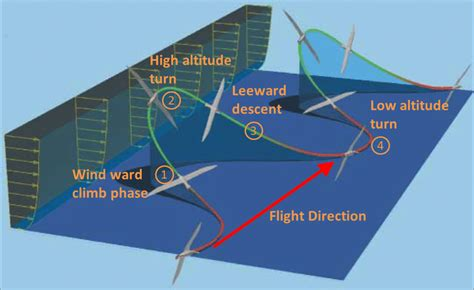
\includegraphics[width=0.5\linewidth]{images/dynamic soaring.jpeg}
    \caption{Dynamic soaring cycle (\textit{https://www.researchgate.net/figure/Dynamic-soaring-cycle_fig1_326672558})}
    \label{fig:Dynamic soaring}
\end{figure}

Next is thermal soaring. During thermal soaring, the albatross flies through or circle in columns of warm air currents that rise from the ground. The rate of descending of the bird is less than the magnitude of the rising air. This makes it possible for the birds to attain more altitude, see Figure (\ref{fig: thermal soaring}). With this extra altitude, the albatross is able to glide to the next thermal (\cite{Evolution_Alba}). 

\begin{figure}
    \centering
    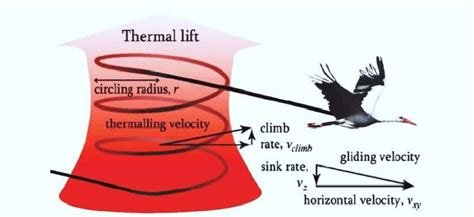
\includegraphics[width=0.5\linewidth]{images/thermal soaring.jpeg}
    \caption{Thermal soaring (\textit{https://www.researchgate.net/figure/Thermal-Soaring-16_fig4_352395064})}
    \label{fig: thermal soaring}
\end{figure}\\

This paper also mentions that even the colors of the wings can have some effect on the endurance of the bird. The temperature difference between the upper (black) and the lower (white) surface of the wings, aids in drag reduction. Temperature plays a significant role in the reduction of induced and skin friction drag.\\

Researchers found that the black-white or black-black wings performed better than the white-black or white-white coloring (\cite{Evolution_Alba}).\\


\subsubsection{What does the Albatrone take from the albatross?} 

Mostly, the shape and the dimensions of the wings. To make the wing structurally sound, the bones in the albatross wing will be taken as inspiration. This is done by having 3D printed joints and the ‘bones’ make out of pieces of balsa wood. The idea is to follow the shape of the wing as best as possible, also making sure the cross section is the same. \\

If possible, the tail feathers of the albatross could also serve as an inspiration for the horizontal stabilizers. For this to work, the placement of the propeller needed to be taken into account.
As told by the expert stakeholder ir. Madeline Zhang, the placement of the propeller has an impact on the stability of the drone. She mentioned that placing the propeller on the back of the drone makes it more stable as it does not cause the airflow over the wings to become turbulent. Placing the propeller in front, means an added risk of the drone back-flipping on take-off. If the propeller is mounted at the back of the Albatrone, the stabilizers should not obstruct the propeller.
 
\begin{figure}
     \centering
     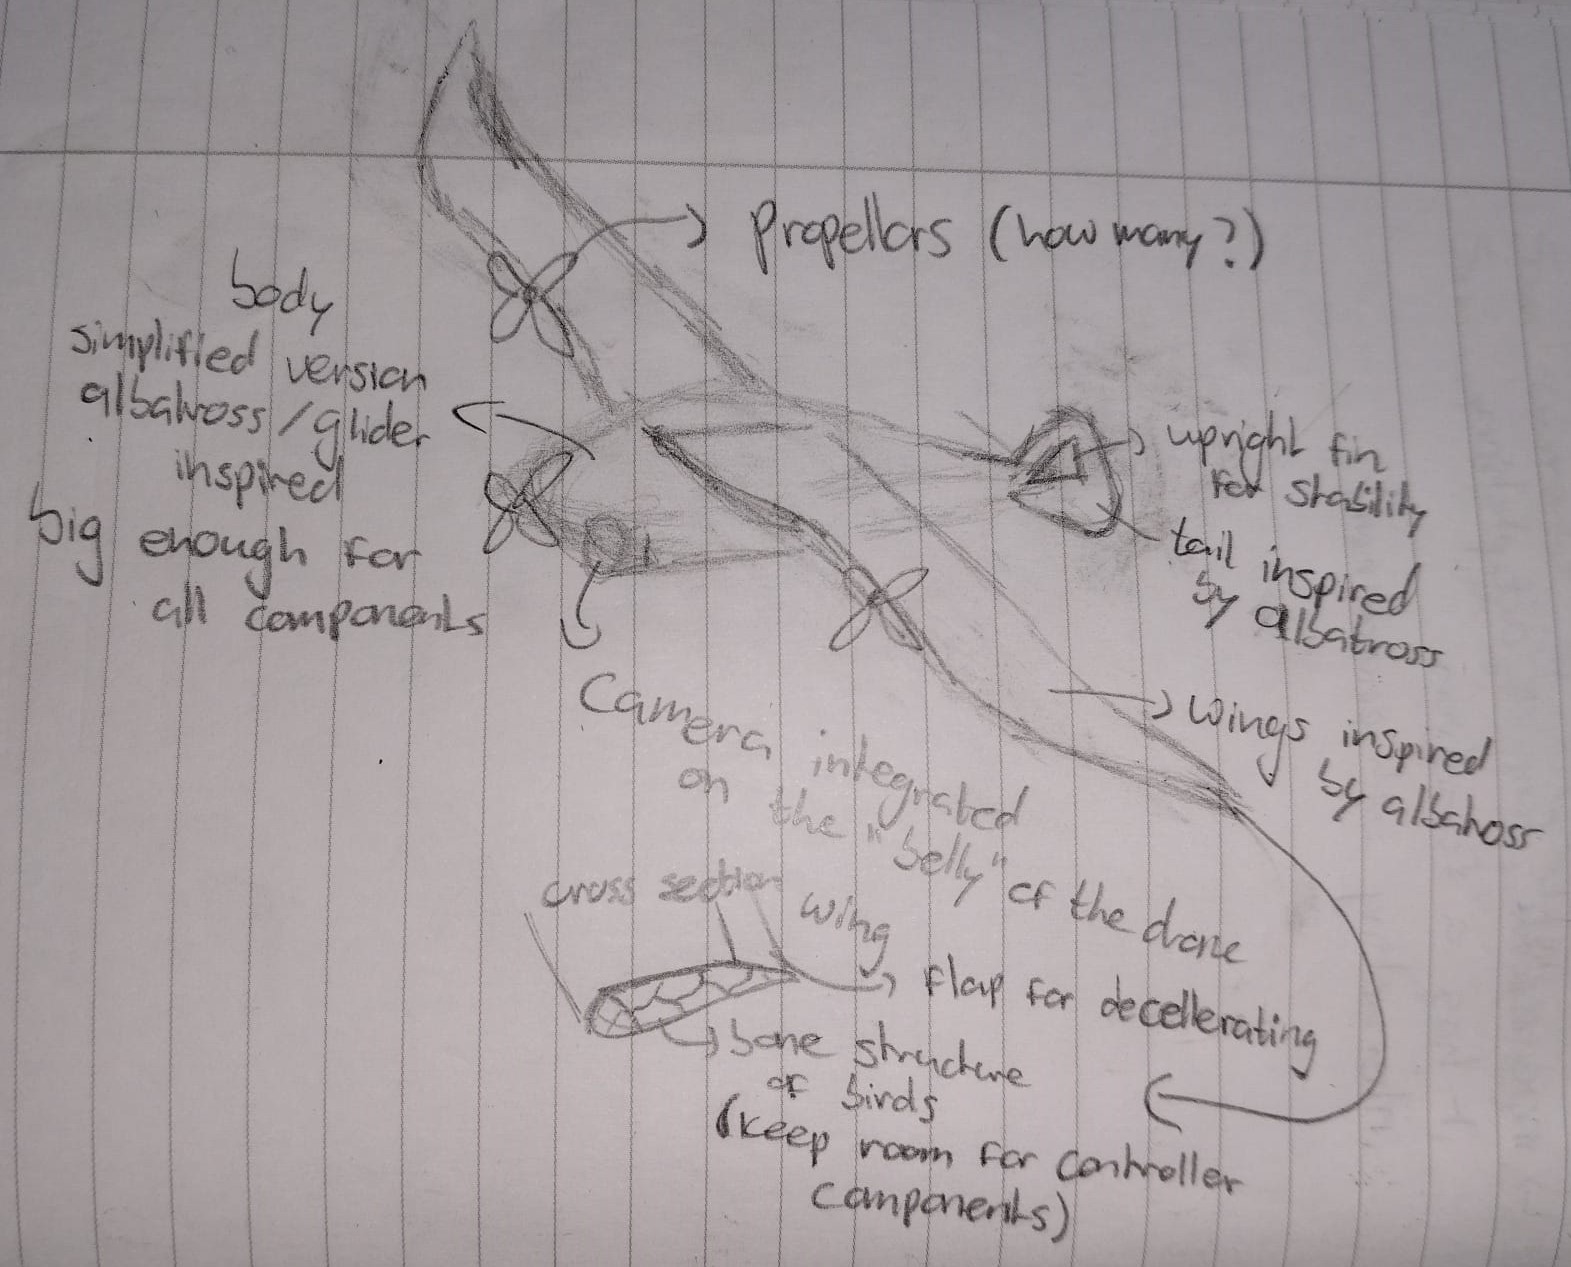
\includegraphics[width=0.5\linewidth]{images/Sketch.jpg}
     \caption{One of the first sketches of the Albatrone}
     \label{fig:Sketch Albatrone}
 \end{figure}

 In figure \ref{fig:Sketch Albatrone}, one of the first sketches of the Albatrone can be seen. Highlighted are the wings, tail, body and bone structure that are inspired by the albatross. \\

 

\section{Design evolution} 

During the time between the project proposal and the final report, some changes occurred. 

 

\subsection{Material} 
In the beginning of this design process, our 'plan A' was to use a Carbonfiber-nylon filament (PAHT-CF). During a meeting with our expert stakeholder Ir. Madeline Zhang, she mentioned that making the Albatrone out of balsa wood and shrink foil would be a good option to keep it lightweight. While making the Albatrone out of wood was an option, the availability and prices online, plus the lack of modes of transportation to get the wood to the Makerspace, made this option not final. The people of the Technology Center also provided feedback during a project standup session. Here they mentioned that balsa wood and shrink foil might not be strong enough to hold the electronics. This lead to researching ways to improve the structural stability. I-beams were an option, but most I-beams are made of metals. A wooden I-beam was really expensive and not made of the lighter balsa wood.

Another option that was presented by the project staff was styrofoam. This option was briefly explored. However, the shaping needed to be done with a foam cutter. This required a steady hand from the cutter and the shape of both wings needed to be the same. Having two identical but mirrored versions of an albatross wing out of styrofoam, seemed unlikely.

With a little more research, a different filament, Bambu PLA Aero, was found to be suitable for the Albatrone. This filament is a sort of "active foaming PLA" specially advertised by use for Remote Controlled Planes (\cite{PLA_Aero}). This change did mean that some different dimensions were needed as every part needed to fit in the BambuLab X1 Carbon or X1E. This also meant that 3D printed 'joints' and wooden 'bones' were no longer needed. While losing this bio-mimicry component, it now became possible to incorporate the hollow bone structure of birds by the configurable sparse infill of those 3D printers. Again, the people from the Technology Center provided feedback. They were a little hesitant at first and mentioned that most plastics had a similar density and could be too heavy for our application. On the other hand, when the properties of the PLA Aero were explained, they became intrigued. This solidified our choice in material.

When ordering the filament, Murphy's law struck again. On the website of `Electronica voor jou', it said that there was one roll of black PLA Aero available. The filament was ordered on the 10th of December, after contacting the business three separate times and waiting for over a month (13th of January), they finally said they could not order this specific PLA. The PLA Aero was ordered by a different business, only this time in white. As mentioned in the 'Background information and research' part, black-white or black-black wings create (even if it is just a little) less drag compared to the white-black or white-white wings. While this color change will most likely not be responsible for big changes in the performance of the Albatrone, especially during winter, it could be interesting to try and recreate these findings on the Albatrone in the future. While waiting for the right filament to arrive, parts of the design was printed using regular PLA. These prints were used to test the way the parts are attached to each other and the tolerances of the BambuLab printers.


\subsection{Wing dimensions} 
Another change, the dimensions of the wings. The biggest chord length was estimated to be around 270 mm for the smaller gray-headed albatross. This was based on an estimation that the wing is roughly 1/3 of the length of the body of the albatross. This estimation came from measuring a picture of the gray-headed albatross from google. 

The length of the body of was found to be in the range of 71 to 82 cm (710 to 820 mm) (\cite{WoRMS}).

To get the top view of the wing, the length of the bones (humerus, ulna, and the manus + primaries) were used to get an idea of how long each part must be (\cite{Wing_shape}). The wingtip is put at a 60 degree angle to make it easier to calculate the area of the wing. 

In the same paper, the aspect ratio of the gray-headed albatross (or the Diomedea chrysostoma), is found to be 15.3. with a wingspan of 200 cm.  

To find the aspect ratio, the wingspan squared is divided by the wing area.\\

To get to an aspect ratio close to this 15.3, the chord length needed to be smaller than expected.\\

Calculating the aspect ratio should be somewhat simple. Unfortunately, it would not be a (school) project without even the smallest things going wrong. A while after using the aspect ratio as a guide on how big the chord length of the different parts of the wing should be and keeping in mind that during this calculation the dimensions of the body was just an estimate, the realization that in all those calculations the area of the body was wrongly calculated came a little too late.\\

As mentioned above, the chord length started at 270 mm. Limited by the dimensions of the 3D printer, this became 250 mm. After realizing the mistake in the calculation of the aspect ratio, the only 'quick fix' that came to mind was to make the first part of the wing shorter both in length and width as the thickness needed to intergrade the servo that controls the ailerons in the middle part of the wing, was set to 145 mm. The maximum chord length ended up being 150 mm which quickly goes to 145 mm for most of the wing.\\

\subsection{Body} 
The journey to the perfect body. In the beginning, the idea was to make the body a more simplified version of that of the albatross. This meant following the general shape of the albatross without the beak. However, designing organic shapes in SolidWorks or Fusion was proven to be tricky as is evident by the first attempt of the wing design in Figure \ref{fig:Fusion wing fail}.\\

\begin{figure}
    \centering
    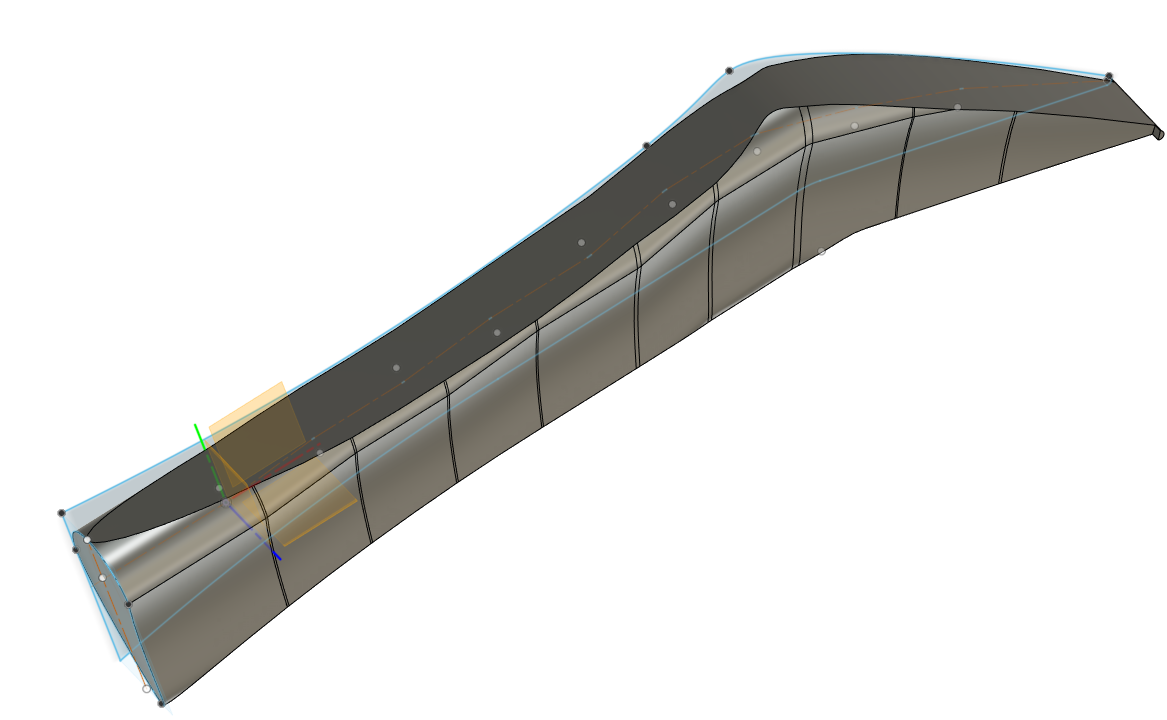
\includegraphics[width=0.5\linewidth]{images/Fusion wing fail.png}
    \caption{First attempt designing the wing in Fusion}
    \label{fig:Fusion wing fail}
\end{figure}\\

To keep the design manageable, the body ended up more cylindrical as can be seen in Figure \ref{fig:Cylindrical body}, but not without trying the other things that came to mind.\\

The first few iterations mostly resembled a bullet shell, see Figure \ref{fig:bullet shell} and \ref{fig:Unfinished bullet}. In the second figure, the idea was to make the walls straight to make it easier for the wings to attach to the body. Figure \ref{fig:Eehm...no} was an attempt to make a symmetrical body with straight walls for the wing attachment. This did not really work. So, a little more thinking was needed before going to SolidWorks.
The resemblance to a bullet occurred most likely because the head and body were attached together. Again, because the limitations of the available printing dimensions, this was not the right approach. \\

To get the desired length of the whole body, the body, head and tail were separated. To make sure the inside of the body could be reached, a part of the body was cut horizontally. Next slots were added to be able to attach the rest of the body to this open part. The head, tail and wings would hopefully keep the body closed during flight. Figure \ref{fig:Cylindrical body} and \ref{fig:Oval top} were designed more carefully.

\begin{figure}
    \centering
    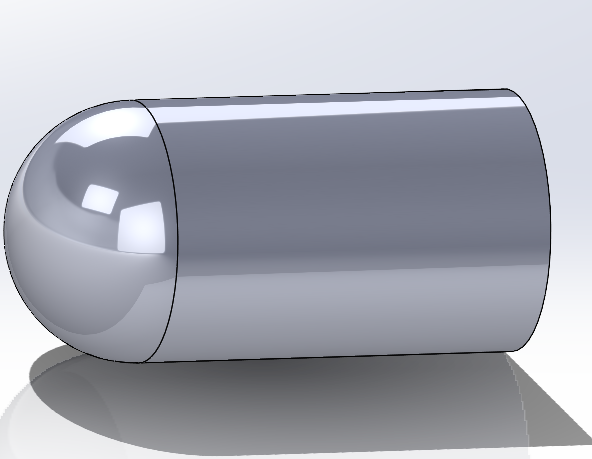
\includegraphics[width=0.5\linewidth]{images/Bullet shell.png}
    \caption{Bullet shell body}
    \label{fig:bullet shell}
\end{figure}

\begin{figure}
    \centering
    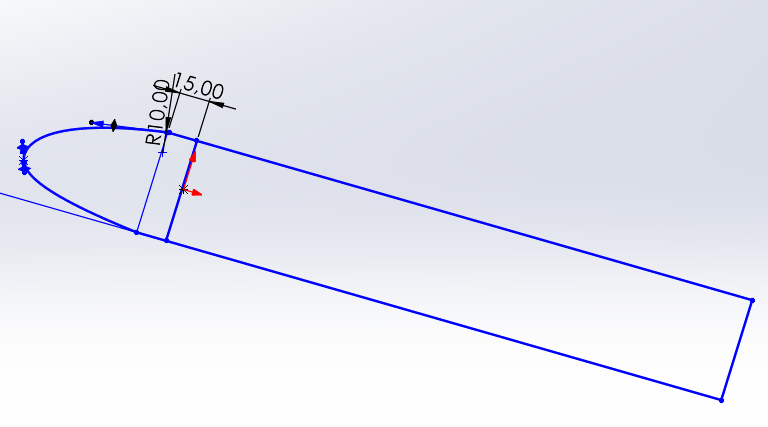
\includegraphics[width=0.5\linewidth]{images/Unfinished bullet.png}
    \caption{Sketch straight-walled bullet body}
    \label{fig:Unfinished bullet}
\end{figure}

\begin{figure}
    \centering
    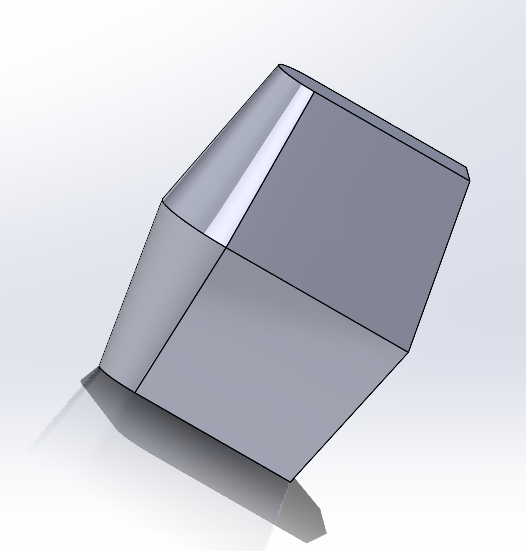
\includegraphics[width=0.5\linewidth]{images/Eehm...no.png}
    \caption{Attempt to make a symmetric, straight-walled body}
    \label{fig:Eehm...no}
\end{figure}

\begin{figure}
    \centering
    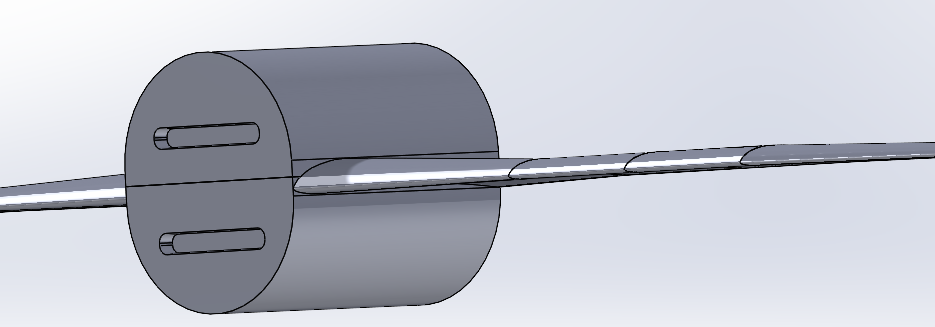
\includegraphics[width=0.5\linewidth]{images/Cylindrical body.png}
    \caption{Cylindrical body}
    \label{fig:Cylindrical body}
\end{figure}

\begin{figure}
    \centering
    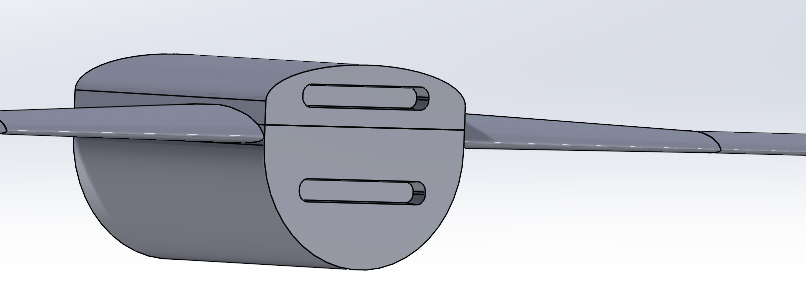
\includegraphics[width=0.5\linewidth]{images/Body oval top.png}
    \caption{Body with oval top}
    \label{fig:Oval top}
\end{figure}


Not only the shape of the body went through some iterations, but also the dimensions. The planned width of the body was around 200 mm to get the wingspan close to the 2 meters from the gray-headed albatross. In the end, this changed. The choice was made to design the body as small as possible, while still being able to hold all the electronics. This decision was based on the insight that the body would most likely only negatively affect the aerodynamics as the bulk of the body would be a cylinder. The design in Figure \ref{fig:Cylindrical body} was first made with a radius of 55 mm on the outside with a wall thickness of 2 mm. This made the whole body quite big in relation to the cross-section of the wings. To save on material, weight and hopefully improve on the aerodynamics, the top was designed to be more oval. This change did not go as smoothly as thought. SolidWorks began moving points when changing the height of the ellipse in the sketch or did not connect the sketch of the ellipse to the right point in the sketch. This made it quite difficult to accurately design the body. After deleting, redrawing, and double checking the sketches again and again, the body did eventually line up. However, in the mean time, the electronic parts had arrived. This meant that is was now possible to design the body more around the electronics. This took away the some of the guesswork with regards to the size needed. With a smaller body, the drag would decrease and the weight would decrease, resulting in better aerodynamic properties. Keeping the issues with the oval top in mind, this smaller body design went back to the two half circles as seen in Figure \ref{fig:Cylindrical body}.

\subsection{Tail} 
The main goal for the tail is to be able to stabilize the drone with the vertical and horizontal stabilizers [https://aerotoolbox.com/design-aircraft-tail/]. The process of designing the stabilizers is explained later. For the shape of the tail of the Albatrone, inspiration was taken from pictures of the tail of planes. Looking at pictures of planes, it was noted that in a lot of pictures, the underside of the tail curves up. Keeping the top line of the plane straight. Figure \ref{fig:Tail v1} shows the first iteration of the tail. Figure \ref{fig:Albatrone small body} shows the tail more in line with the top of the body.\\

\begin{figure}
    \centering
    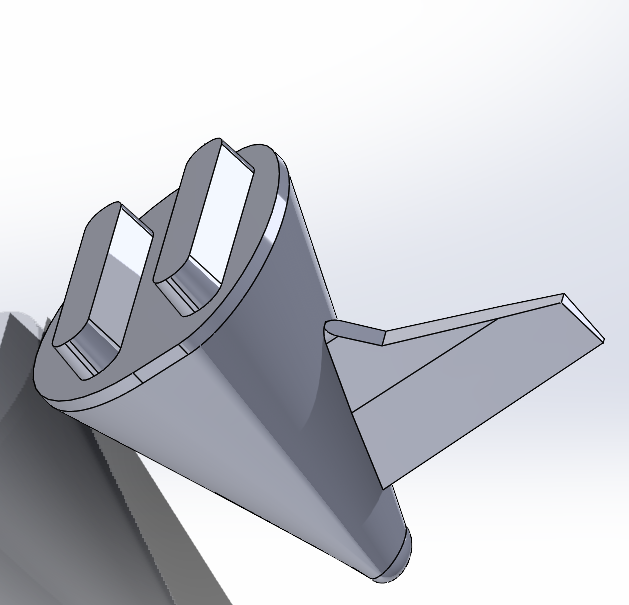
\includegraphics[width=0.5\linewidth]{images/Tail v1.png}
    \caption{Tail design more centered on the body}
    \label{fig:Tail v1}
\end{figure}

\begin{figure}
    \centering
    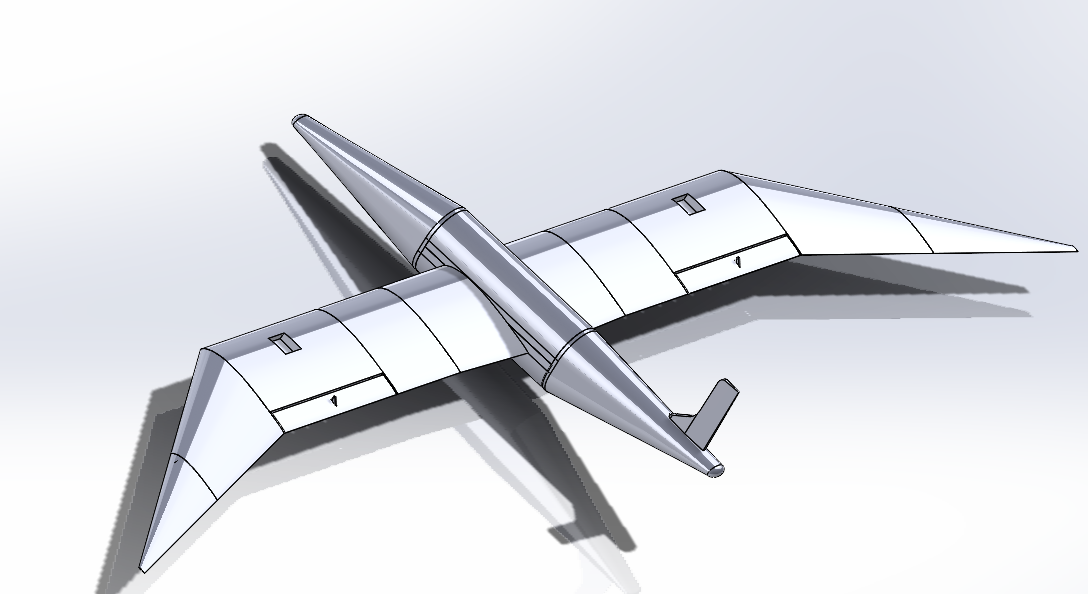
\includegraphics[width=0.5\linewidth]{images/Albatrone small body.png}
    \caption{Albatrone where tail is more in line with the top of the body}
    \label{fig:Albatrone small body}
\end{figure}

\subsection{Head} 
As mentioned before, first the design for the head mostly resembled a bullet shell. When it became clear the body also needed to be printed in sections, the head of the Albatrone became more of a cone shape, similar to the tail, as can be seen in Figure \ref{fig:Albatrone small body}. However, this was mostly due to a lack of knowledge on how to create a more plane-like nosecone, With the help from a YouTube tutorial called 'Solidworks Loft Basics - Design an Aircraft Nosecone (CAD Tutorial for Beginners! - B737 \& F-22)' from VDEngineering, the nosecone became more similar to a 'normal' nosecone from a plane (\cite{Nosecone}). To follow this tutorial, a side, top, and front view was needed. This, unfortunately, meant that it was not possible to just use any picture. To still keep the spirit of using the albatross, a blueprint of the Aero L-39 Albatros was used to design the head (\cite{DrawingNC}). With the help of the tutorial, the head now looked as in Figure \ref{fig:Plane nose}. The choice of the plane was purely based on the name and which plane seemed to have a pointier nose as to mimic the beak of the albatross even if it is just a little. If time had allowed, it would be possible to create multiple noses and see which one worked better. Unfortunately, this was not possible in the time that was left for the project.\\

\begin{figure}
    \centering
    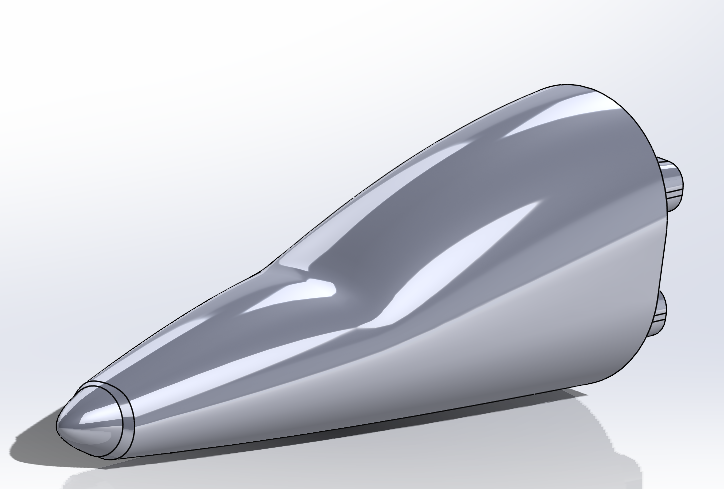
\includegraphics[width=0.5\linewidth]{images/Plane nose.png}
    \caption{Head inspired by the Aero L-39 Albatros}
    \label{fig:Plane nose}
\end{figure}
\\

\subsection{Control surfaces}
To be able to control the drone, control surfaces are needed. An overview of the control surfaces of a plane can be seen in Figure \ref{Control surfaces} For the wings this meant that one middle part needed a flap to be able to manipulate the airflow around the wing (ailerons). At first, to test if it was possible, a small rectangular grove was cut out of the wing. This resulted in a totally detached flap that needed to be accurately positioned on both sides of the wing to keep symmetry. Next, the idea was to keep the upper part of the flap attached to the wing and making the cut on the bottom at an angle to make it able to go down. This would fix the problem of the positioning but decreases the mobility. Also, this idea would take some trial and error as the thickness of the connection would determine the force needed to move the flap. The higher the force needed to move the flap, the more powerful (and most likely bigger and heaver) the servo needs to be.\\

\begin{figure}
    \centering
    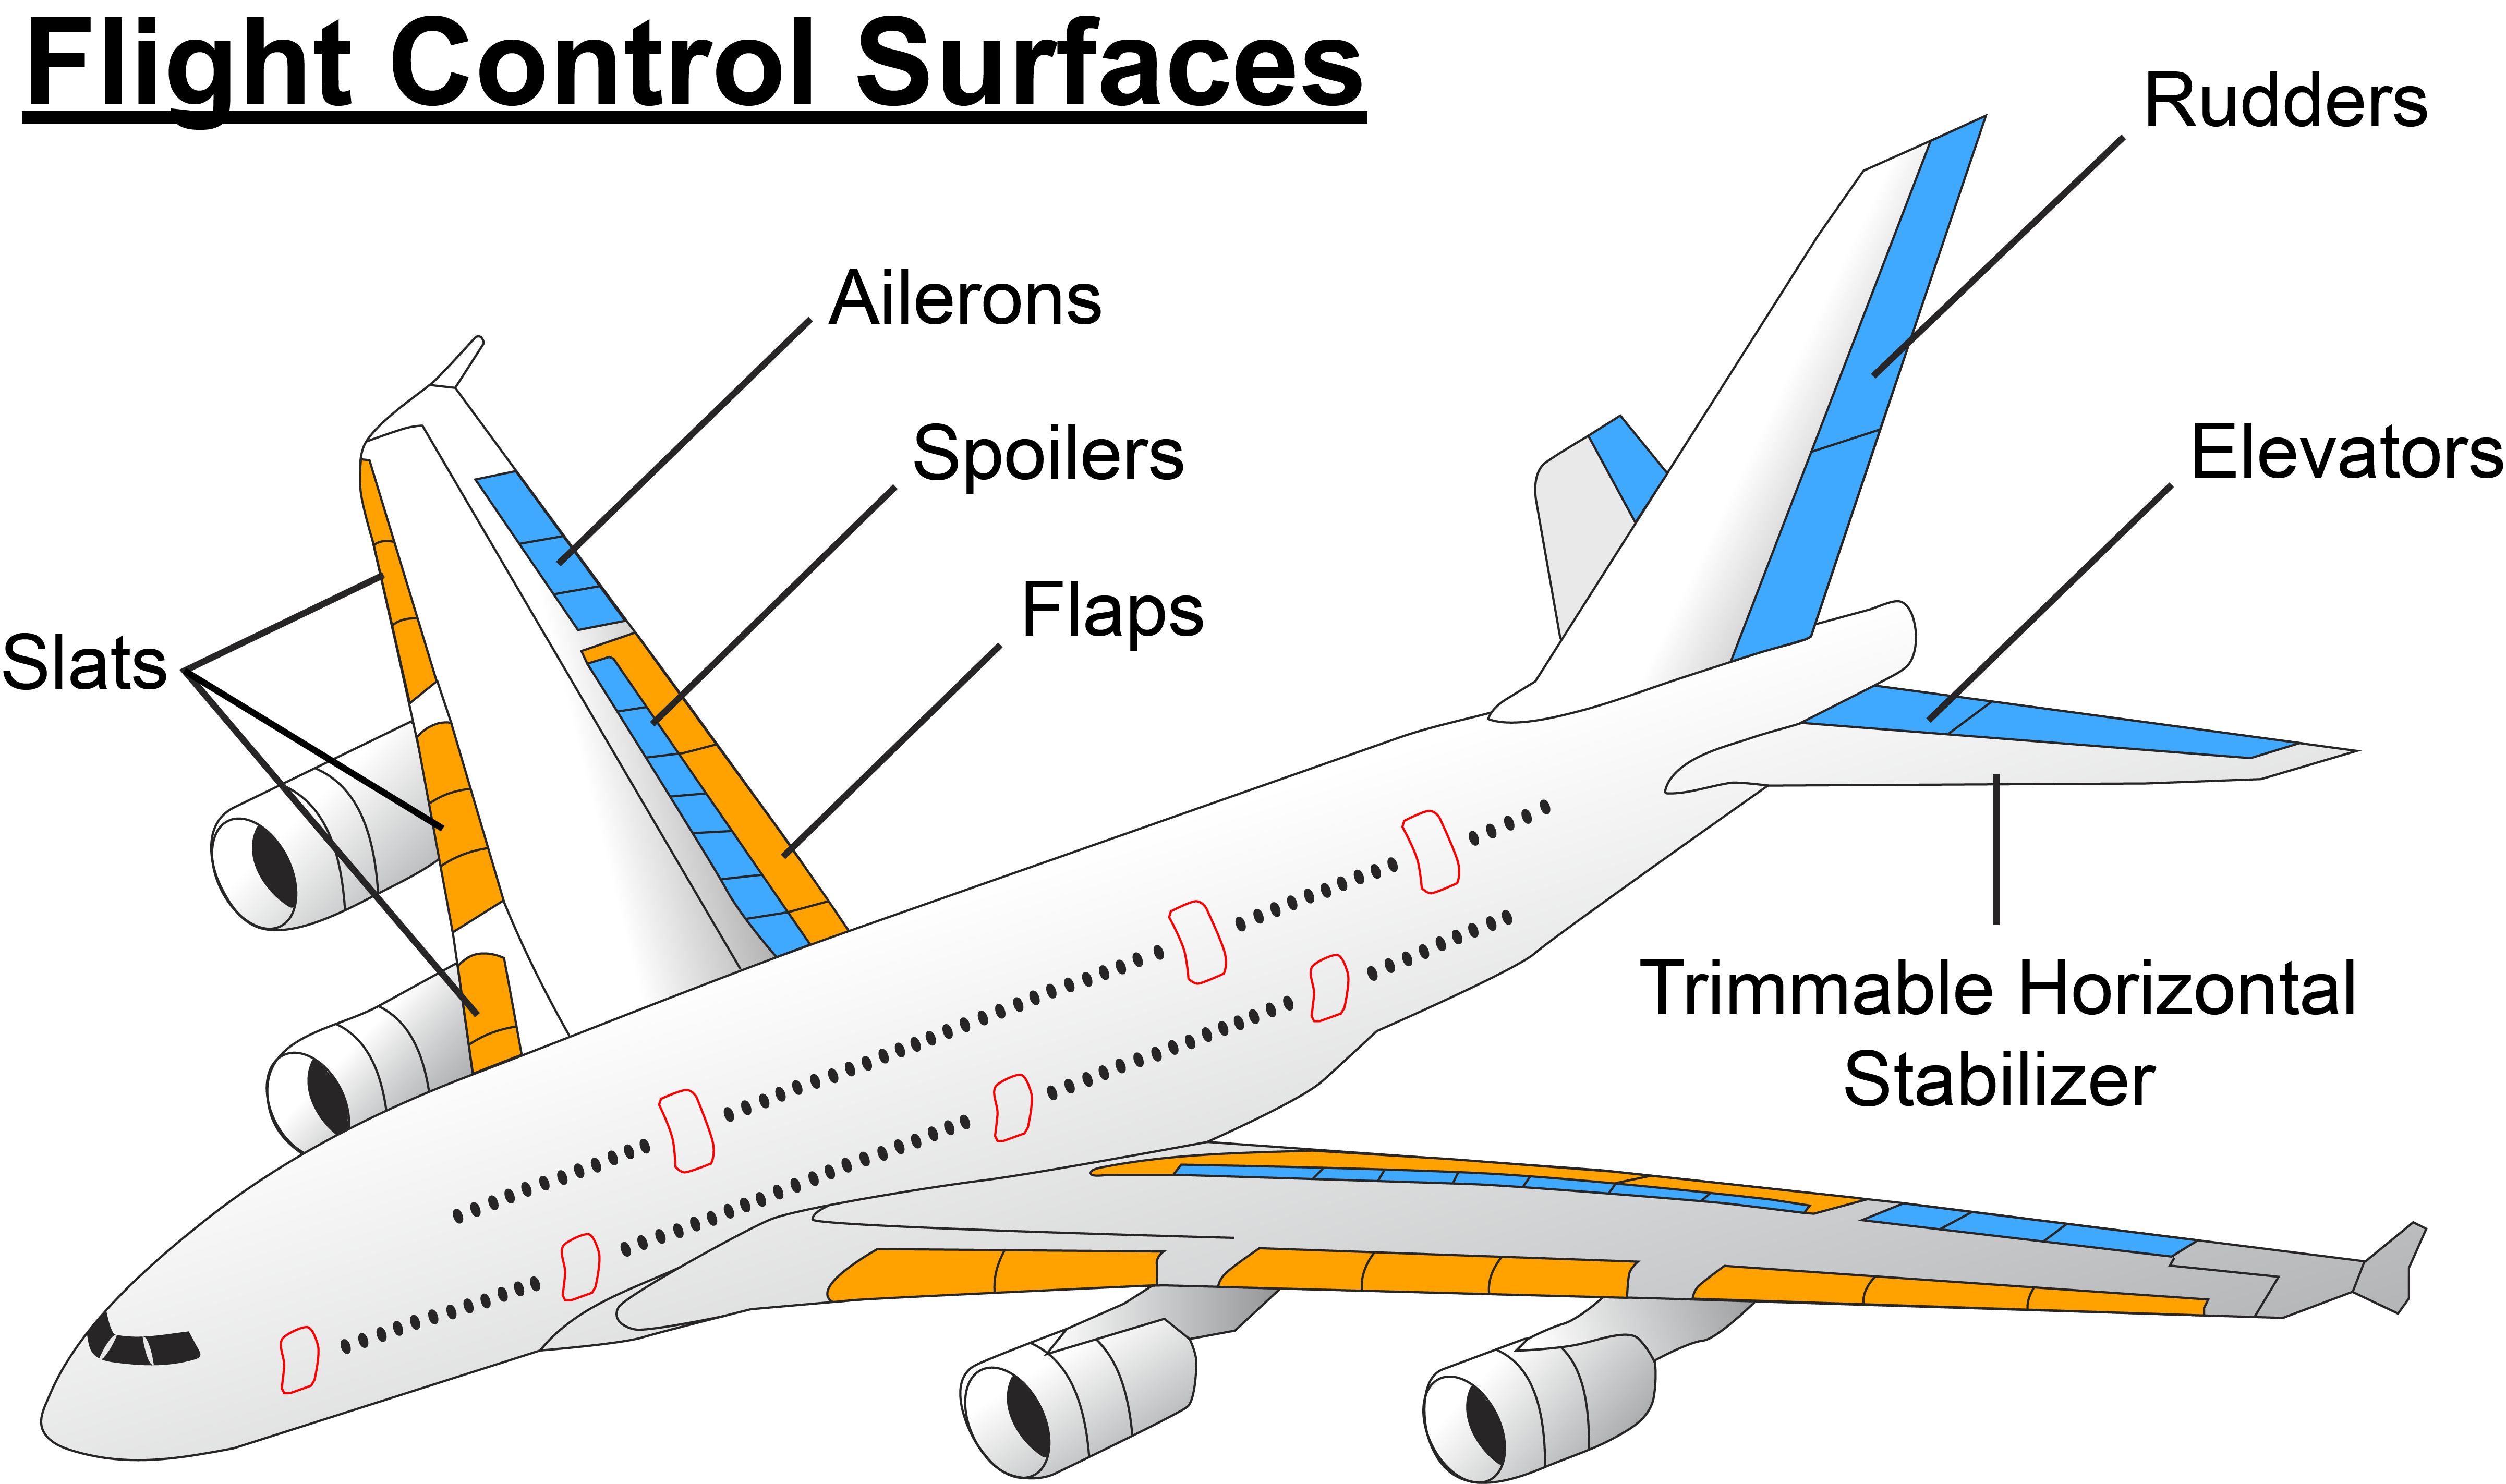
\includegraphics[width=0.5\linewidth]{images/Control surfaces.png}
    \caption{Overview of the control surfaces of a plane (\textit{https://www.naii.com/DesignExamples/TestingAircraftControlSurfaces})}
    \label{Control surfaces}
\end{figure}

Eventually, the design is based on a tutorial found on youtube.com called 'Solidworks | Wing control surface animation | Aileron animation in solidworks' by Rao Aerospace (\cite{Aileron}). In this design the aileron is attached to the rest of the wing with a rod. For the Albatrone, a longer skewer should do the trick.

As for the vertical stabilizer, the first attempt was just a rectangle on the tail. After taking some inspiration from google images on tails of planes, there was an attempt to make it a little more aerodynamic. This resulted in the design in Figure \ref{fig:Sketchy vertical stab}.

\begin{figure}
    \centering
    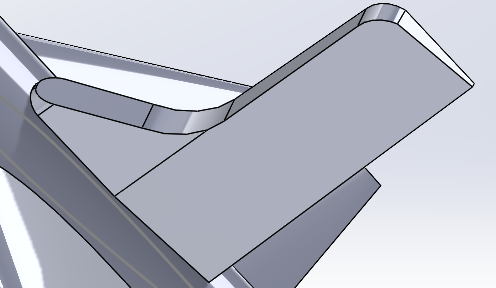
\includegraphics[width=0.5\linewidth]{images/Sketchy vertical stab.png}
    \caption{Attempt at making the vertical stabilizer more aerodynamic}
    \label{fig:Sketchy vertical stab}
\end{figure}

Realizing the horizontal stabilizers are quite important as they make sure a plane is stable during a flight, more research needed to be done. First, another expert stakeholder, a neighbor of one of the members of the team (Romy) and an retired pilot that sails as a hobby, was nice enough to lend out his study books on planes, high-speed aerodynamics, and even one on the aero-hydrodynamics of sailing. While being very interesting, these books talked more about how to control a plane and not really on the design of the plane. However, during the talk with the neighbor, he advised to use the a wind tunnel to figure out what design works better and could be implemented in the design. He mentioned that calculations are nice, but some things cannot be calculated. Therefor, having access to a wind tunnel and analyzing the results, was more useful. Again, if time had allowed, adding different stabilizers to the Albatrone and noting the difference in the stability, would be ideal.

Focusing on the design of the stabilizers, a google search lead to a more useful page on Aircraft Horizontal and Vertical Tail Design (\cite{Stablizers}). This page mentions the different configurations, a relation to calculate the minimum area of the stabilizers based on some parameters from both the wing and the horizontal stabilizer itself. This page also presented an answer on the question what shape could be used for the stabilizers. A very common choice is apparently either the NACA 0010 or NACA 0012 airfoil. Comparing these airfoils again on airfoiltools.com, the NACA 0012 looks to be a little more stable than the NACA 0010, thus the decision on the airfoil for the horizontal stabilizers was made. Figure \ref{fig:Horizontal stab} shows the end result of hours full of struggling with lofts, deleting and redrawing the sketch of the curves on the sketch plane, and checking again and again if the two stabilizers are in fact symmetric and placed at the same location on the tail. At the time of writing, the elevators and the corresponding servo attachment and designated servo spot are not yet implemented.

Because this airfoil is most likely more aerodynamic than the vertical stabilizer seen in Figure \ref{fig:Sketchy vertical stab}, this airfoil will also be used as the vertical stabilizer (not yet implemented at time of writing).

\begin{figure}
    \centering
    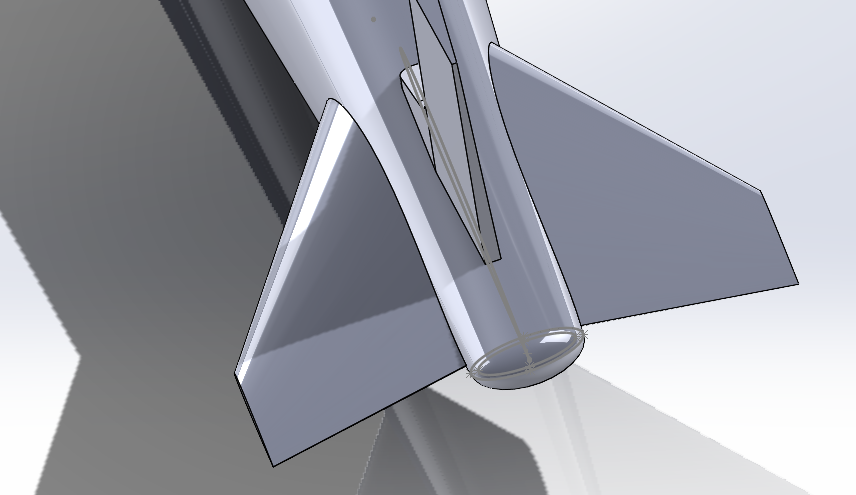
\includegraphics[width=0.5\linewidth]{images/Horizonal stab.png}
    \caption{Horizontal stabilizers}
    \label{fig:Horizontal stab}
\end{figure}\\

\subsection{Connections}
It should not come as a surprise that the Albatross is made of separate parts. All those separate parts need to be connected. The connection between the different parts of the wing was quickly designed.The people of the Technology Center were not entirely sure these connections would hold up because of the stress concentrations created by such a connection. However, when testing the connections when printed with regular PLA, they proven to be strong enough to withstand the not-so-scientific stress test called 'trying our best to break them using our hands'. Another option, more in the direction of duck tails, see Figure \ref{fig:T-ducktails} was also tested. The test print looked as in Figure \ref{fig:Attachment test}. As the tolerance on these test prints was too large for our application, this idea was scrapped. 

\begin{figure}
    \centering
    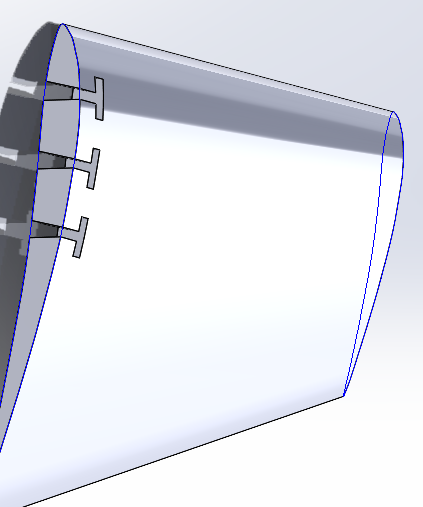
\includegraphics[width=0.5\linewidth]{images/T ducktails.png}
    \caption{T-shaped duck tail inspired attachment method}
    \label{fig:T-ducktails}
\end{figure}\\

\begin{figure}
    \centering
    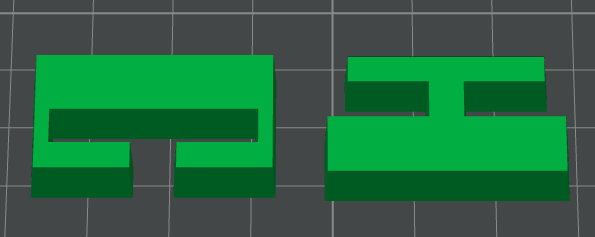
\includegraphics[width=0.5\linewidth]{images/Attachment test.png}
    \caption{Test print T-shaped ducktails}
    \label{fig:Attachment test}
\end{figure}

The connection between the wing and the body required a little more thought. To test the best angle of attack for the Albatrone's wings, this attachment needed to allow one degree of freedom, the rotation. To allow for this rotation, a pin and hole connection was implemented; see Figure \ref{fig:Body pin connection}. Also visible in this figure are the connections between the other parts of the body (see \ref{fig:Tail v1} for the other part of the connection)

\begin{figure}
    \centering
    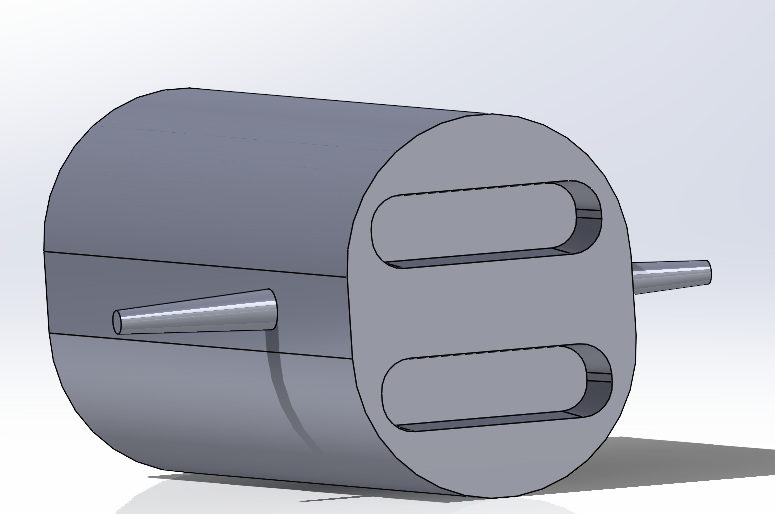
\includegraphics[width=0.5\linewidth]{images/Body pin connection.png}
    \caption{Body with pin to connect to the wing}
    \label{fig:Body pin connection}
\end{figure}

As described above, this middle part of the body is cut in two to make it easy accessible. These two parts are held together by the pin-hole connections between the body and the wing and also by the extrusion and hole slots in the extra body parts made in order to get the desired length.\\

\subsubsection{Final design}
After implementing aforementioned design choices, the current final design can be seen in Figure \ref{fig:Final design}. The horizontal and vertical stabilizers are not finished yet. The horizontal stabilizers need elevators and room for the servo. The vertical stabilizer will be changed to the NACA 0012 airfoil. At the time of writing, the printing of the Albatrone is not done and is therefor also not tested. If in the next few days changes need to be made, this will obviously not be recorded in this specific report.

\begin{figure}
    \centering
    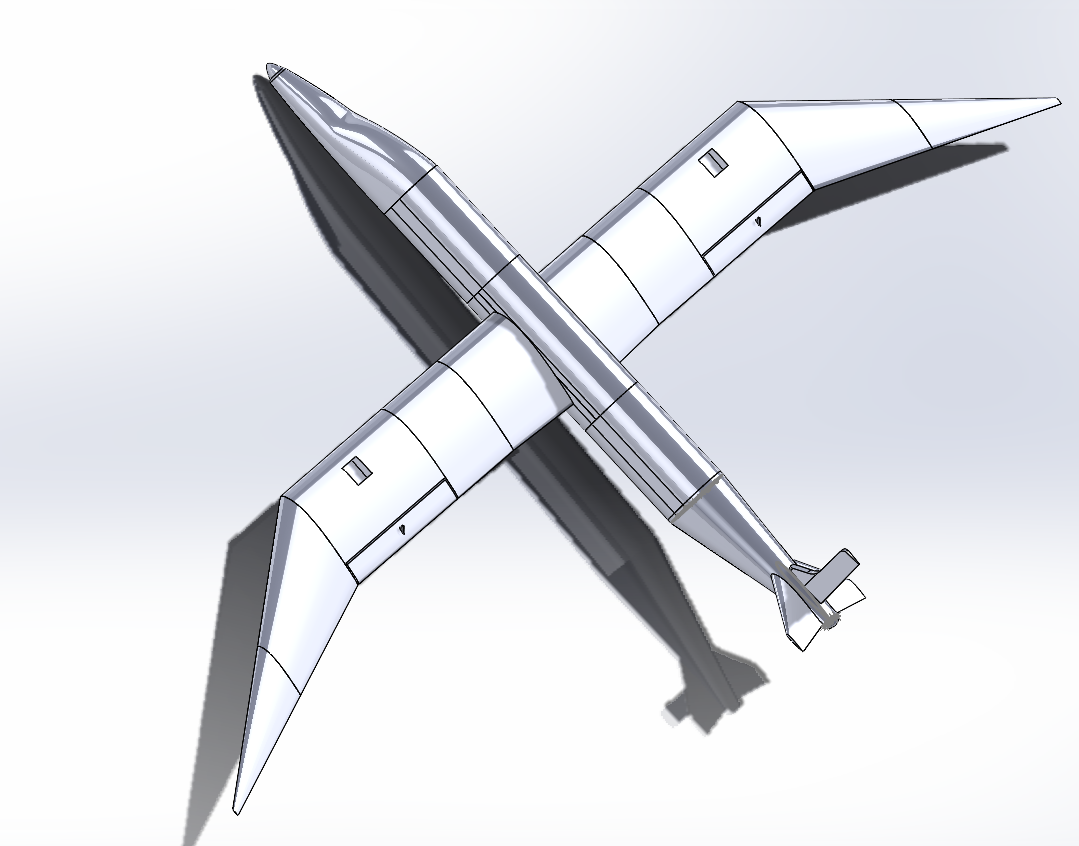
\includegraphics[width=0.5\linewidth]{images/Final design.png}
    \caption{Final design}
    \label{fig:Final design}
\end{figure}

\subsection{Stakeholders}
As briefly touched upon in the text above, some design changes were made due to feedback or insights from stakeholders.

In the morning of November the 4th, we had a meeting with a police detective and specialist on the drones unit. Before the meeting, the idea was to use a combination of Lidar and Radar to obtain information about the surrounding. He explained to us that a simple camera can be enough. The power of machine learning is so powerful, that the algorithm can help more than enough. He also redirected us to an initiative called Avy. Avy makes the drone and finishes the paper work, so that the police can buy it and use it immediately. Avy was not responsive for a long period of time, but it was managed to make an appointment in the week of the presentations.

In the afternoon of November 18th, one of the members of the team attended the opening of E.N.G.A.G.E. which is the first so-called gameroom in the Department of Defense. It was organized by the "Korps Mariniers", and there were a lot of demos at the location. One of those demos was about Unmanned Aerial Systems (UAS), by the Head Coordinator of the Marine training center. I told him about our project, and we exchanged contact information. Around 10 days later we got an email cc'd from him, asking a colleague if he knew someone to help us out. 10 more days later, he responded and we were referred to someone else. This started a chain of replies and forwards, and January 20th we ended up with a specialist from the UAS programme inside the department of Innovation. Unfortunately we haven't had any response as of writing this report.

In the evening of 3 January 2025, a neighbor of one of the members was available for a talk about the Albatrone. This neighbor is a retired pilot and sails as a hobby. As this was during the Christmas break, she went alone. During this talk, the SolidWorks parts, that were finished at the time, were presented. As this neighbor has a lot of knowledge regarding the handeling of and the aerodynamics around a plane, some different design choices made in different planes, specifically KLM (Koninklijke Luchtvaart Maatschappij voor Nederland en Koloniën N.V.) planes and their impact on the aerodynamics were discussed. After this nice talk, the neighbor was kind enough to lend out some older books about piloting and what happens around an aircraft during flight. Also another book about the aero-hydrodynamics was also handed out, just in case.